\section{Aufbau des Systems}
\subsection{Hardwareaufbau}
Ein Steuerrad, drei Pedalen, ein Schaltknüppel und diverse Knöpfen dienen als Eingabegeräte für den Fahrsimulator. Diese sind über USB mit einem Computer verbunden. Als Ausgabe dient ein leistungsstarker Projektor, der das Bild auf eine hochreflektierende Projektionsfläche projiziert.

\begin{figure}[H]
\centering 
\includegraphics[width=0.8\linewidth]{src/foto_hardware_aufbau.png}
\caption{Hardwareaufbau mit Steuerrad und Pedalen} % Titel der Grafik
\label{Hardwareaufbau} % Labelname
\end{figure}

\newpage

\subsection{Systembeschreibung}

% Bild für Systembeschreibung
\begin{figure}[H]
\centering 
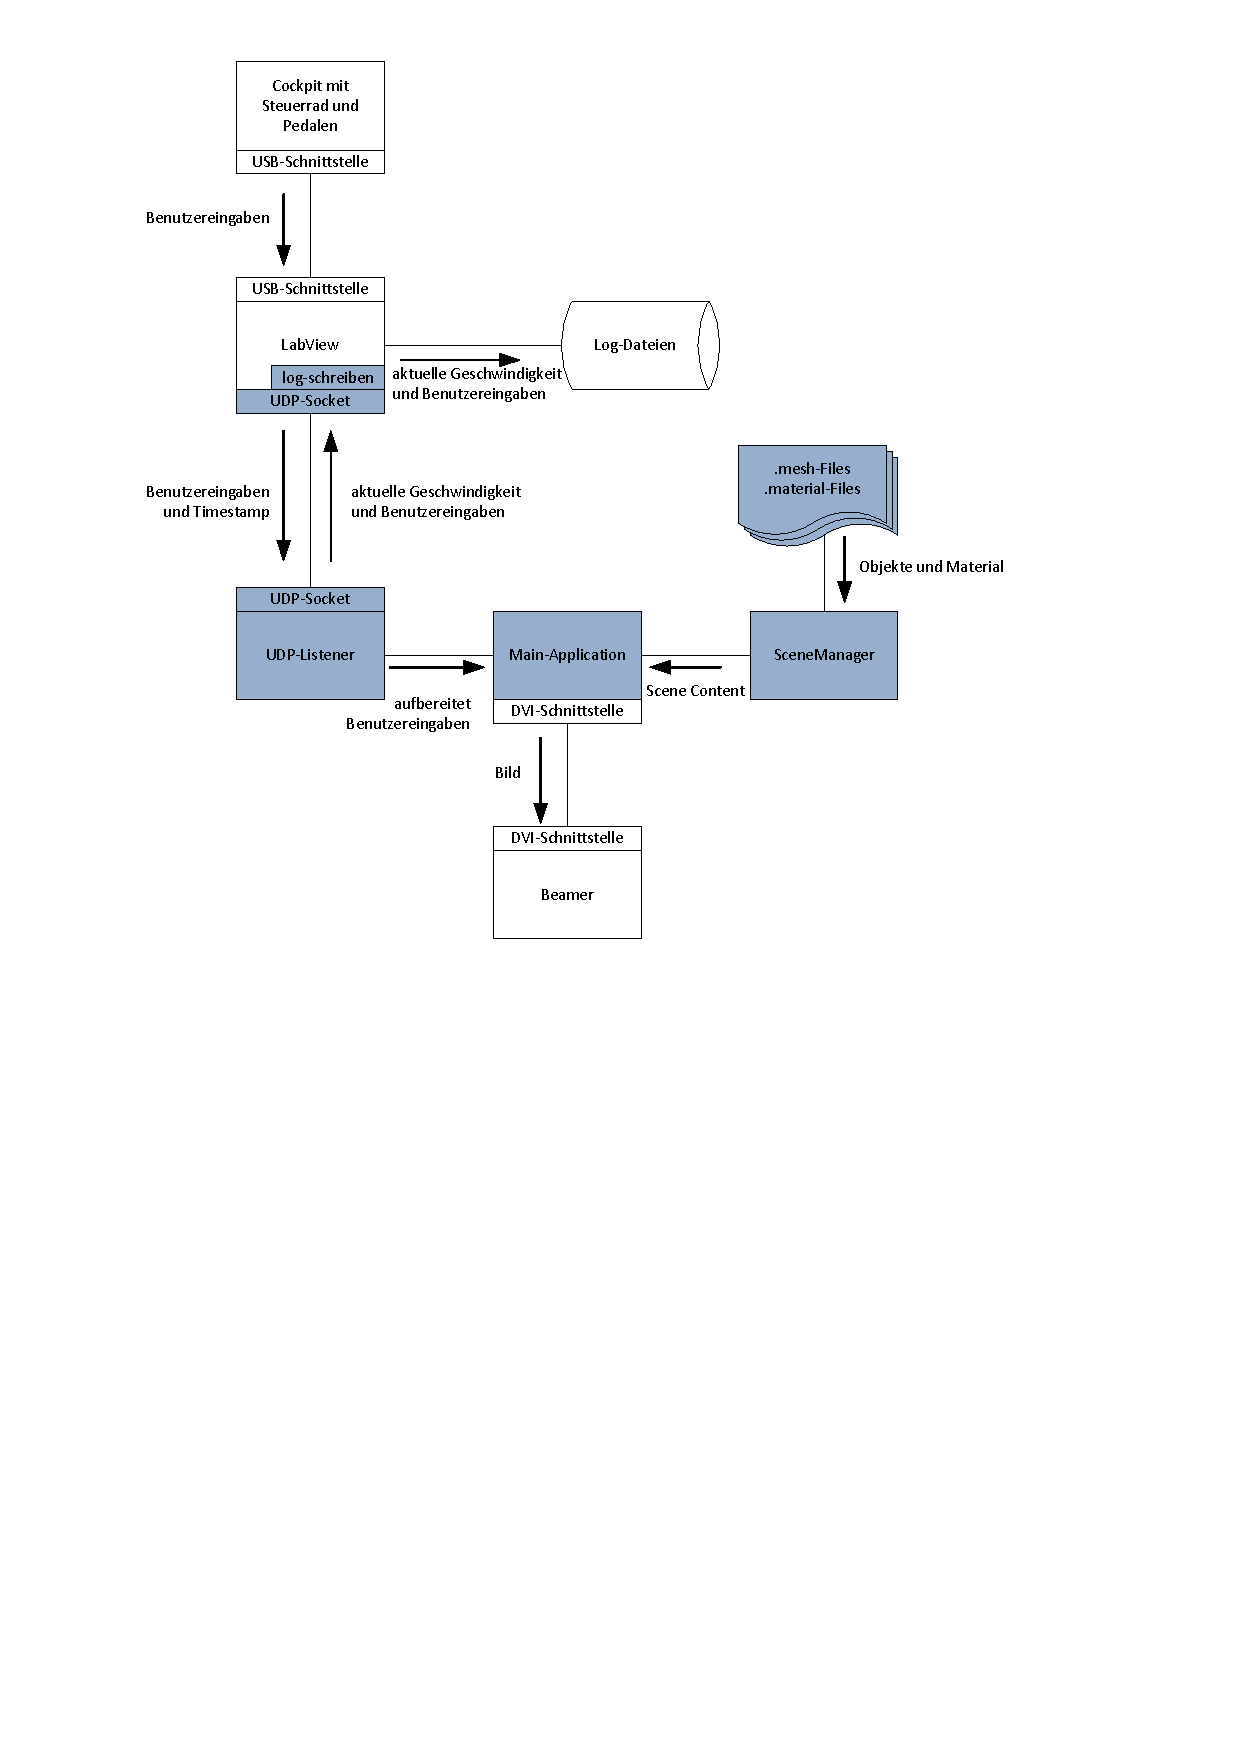
\includegraphics[width=1\linewidth]{src/Systembeschreibung.pdf}
\caption{Systembeschreibung} % Titel der Grafik
\label{Systembeschreibung} % Labelname
\end{figure}

Der Aufbau des Systems für den Fahrsimulator wird anhand der Abbildung \textbf{Systembeschreibung} illustriert. Die blau markierten Komponenten werden im Rahmen dieser Projekt-Arbeit entwickelt. Alle übrigen sind bereits vorbestehend. \\
Benutzereingaben, die im Cockpit gemacht werden, werden von einem LabView Programm eingelesen. Nun benötigt es einen UDP-Port,  über den verschiedene Eingaben an das Programm weitergeleitet werden. Es handelt sich hierbei um Werte, die das Drehen des Steuerrades und den Druck auf Gas- oder Bremspedal quantifizieren. Zusätzlich wird der UDP-Port auch für das Empfangen diverser Log-Daten, die von unserem Programm gesendet werden, verwendet. Die empfangenen Daten werden vom LabVIEW-Programm  in ein Log-File gespeichert.\\
Weiter muss in der Programmiersprache C++ ein UDP-Socket mit entsprechendem UDP-Listener implementieren werden, um die Benutzereingaben zu empfangen. Der UDP-Listener wird gleichzeitig dazu verwendet, die Geschwindigkeit des Fahrzeugs sowie Timestamps und weitere Daten an das LabVIEW Programm zurück zu schicken. Damit können die Daten gespeichert und später ausgewertet werden.\\
Diese Aufteilung durch eine Netzwerkschnittstelle ermöglicht es,  das System, wenn notwendig, zu dezentralisieren. Einfachheitshalber wird der UDP-Listener erst in einem Video-Beispiel implementiert und getestet (Siehe Anhang B). Nachfolgend wird er in das Programm des Fahrsimulator transferiert.\\
Sind die Daten vom UDP-Listener empfangen und aufbereitet, werden sie im Hauptprogramm weiter verwendet. Während die Position des Steuerrades, des Gas- und Bremspedales vom UDP-Listener permanent an das Hauptprogramm übertragen werden, wertet dieses die Positionen aus und veranlasst die entspechenden Aktionen in der geladenen Szene. 
Die Szene selbst wird von einem Szenen-Manager geladen. Die berechnete Szene wird schlussendlich in einem Fenster vom Hauptprogramm angezeigt und über eine DVI-Schnittstelle an den Beamer übertragen. Der Beamer projeziert das Bild an die Wand, die sich direkt vor dem Cockpit befindet. 

\subsection{Anforderungen}
\subsubsection{Funktionale Anforderungen}
\begin{itemize}
\item Der Fahrsimulator ermöglicht es dem Probanden, vom Cockpit aus das Fahrzeug zu steuern. Der Proband blickt durch die Frontscheibe des Fahrzeuges und fährt auf Strassen.
\item Die aktuelle Geschwindigkeit des gesteuerten Fahzeuges soll für den Probanden ersichtlich sein. 
\item Es sollen dem Fahrsimulator zwei Szenen zur Verfügung stehen. Die eine Szene stellt eine Stadt dar, die andere Szene eine Berglandschaft mit Tunnels.
\item Die Manipulationen des Benutzers und wichtige Parameter wie z.B. Geschwindigkeit sollen in einer Datei chronologisch und laufend abgespeichert werden, um diese auszuwerten.
\item Alle ein- und ausgehenden Parameter des System sollen jederzeit im LabVIEW abrufbar sein.
\end{itemize}

\subsubsection {Nicht funktionale Anforderungen}
\renewcommand{\labelenumi}{\alph{enumi})}

\begin{itemize}
\item Das System ist robust. Es muss gegen Fehlereingaben immun sein. 
\item Das Starten des Fahrsimulator sollte möglichst einfach gehalten werden.
\item Das Fahrgefühl des Simulators ist möglichst realitätsnah.
\item Der Fahrsimulator bietet dem Probanden eine möglichst realistische Fahrsimulation, inklusive Strassen, Gebäude und Verkehrsschilder. 
\item Die Reaktionszeit des Systems ist möglichst kurz. Die Verzögerungen sind mess-  und kalkulierbar.
\item Das System ist möglichst modular aufgebaut, um später einfach erweitert werden zu können.
\item Das System funktioniert auf der existierender Hardware, und muss auch lauffähig sein, wenn Teile des Fahrsimulators ausgetauscht werden. 
\end{itemize}
